\chapter{設計と実装}
\label{chap:poordirection}

\section{提案手法}
本研究では,P2P型端末通信フレームワークであるAllJoynを用いて端末間のビーコン情報共有を行う.
具体的には,端末Aで周囲のビーコンを検知し,端末BにビーコンのUUID,RSSIなどの情報を送信する.
また,自身で検知したビーコンの情報と,他端末から送信されたビーコンの情報を保持する.
今回の設計では,同一アクセスポイント内に全ての端末があることを想定している.

\section{開発環境}
本研究では,対象OSをAndroidとし,Android OSで動作するアプリケーションを作成する.
なお,Android 4.3以上かつBluetooth4.0以上に対応した端末を想定している.
\begin{itemize}
\item 開発環境
\begin{itemize}
\item Eclipse 3.8 for Mac OS X
\item Android SDK Tools 23.0.5
\item AllJoyn Android v14.02
\end{itemize}
\item 使用端末
\begin{itemize}
\item TORQUEG01
\item ARROWS NX F-05F
\end{itemize}
\end{itemize}

使用した端末のスペックは以下の通りである.
\begin{table}[htbp]
\centering
\begin{tabular}{|c|c|} \hline
OS &  4.4.2 \\ \hline
CPU & MSM8928 1.4GHz クアッドコア \\ \hline
ROM & 16GB \\ \hline
RAM & 2GB \\ \hline
Bluetooth & Ver.4.0 \\ \hline
Wi-Fi & IEEE802.11a/b/g/n/ac \\ \hline
\end{tabular}
\caption{スペック:TORQUE G01}
\end{table}

\begin{table}[htbp]
\centering
\begin{tabular}{|c|c|} \hline
OS &  4.4.2 \\ \hline
CPU & MSM8974 2.3GHz クアッドコア \\ \hline
ROM & 32GB \\ \hline
RAM & 2GB \\ \hline
Bluetooth & Ver.4.0 \\ \hline
Wi-Fi & IEEE802.11a/b/g/n/ac \\ \hline
\end{tabular}
\caption{スペック:ARROWS NX F-05F}
\end{table}


\section{AllJoynAppの概要}
iBeaconから発せられるビーコンを受信し,AllJoynを用いてビーコン情報を送受信するAndroidアプリであるAllJoynAppを作成する.


\subsection{設計}
今回作成するAllJoynAppには,ビーコンを検知し,AllJoynを用いてビーコン情報を送信するAllJoynClientと,ビーコン情報を受信するAllJoynService,インターフェースを記述したSimpleInterfaceという三つのプログラムがある.
AllJoynServiceはバックグラウンドで動作するプログラムであり,AllJoynClientから呼び出されて起動する.
更に,FINDボタンとSCANボタン,ListViewといったUI部品がある.


\subsection{AllJoynセッション}
今回設計したAllJoynAppのセッションの流れは以下の通りである.

\begin{figure}[htbp]
\centering
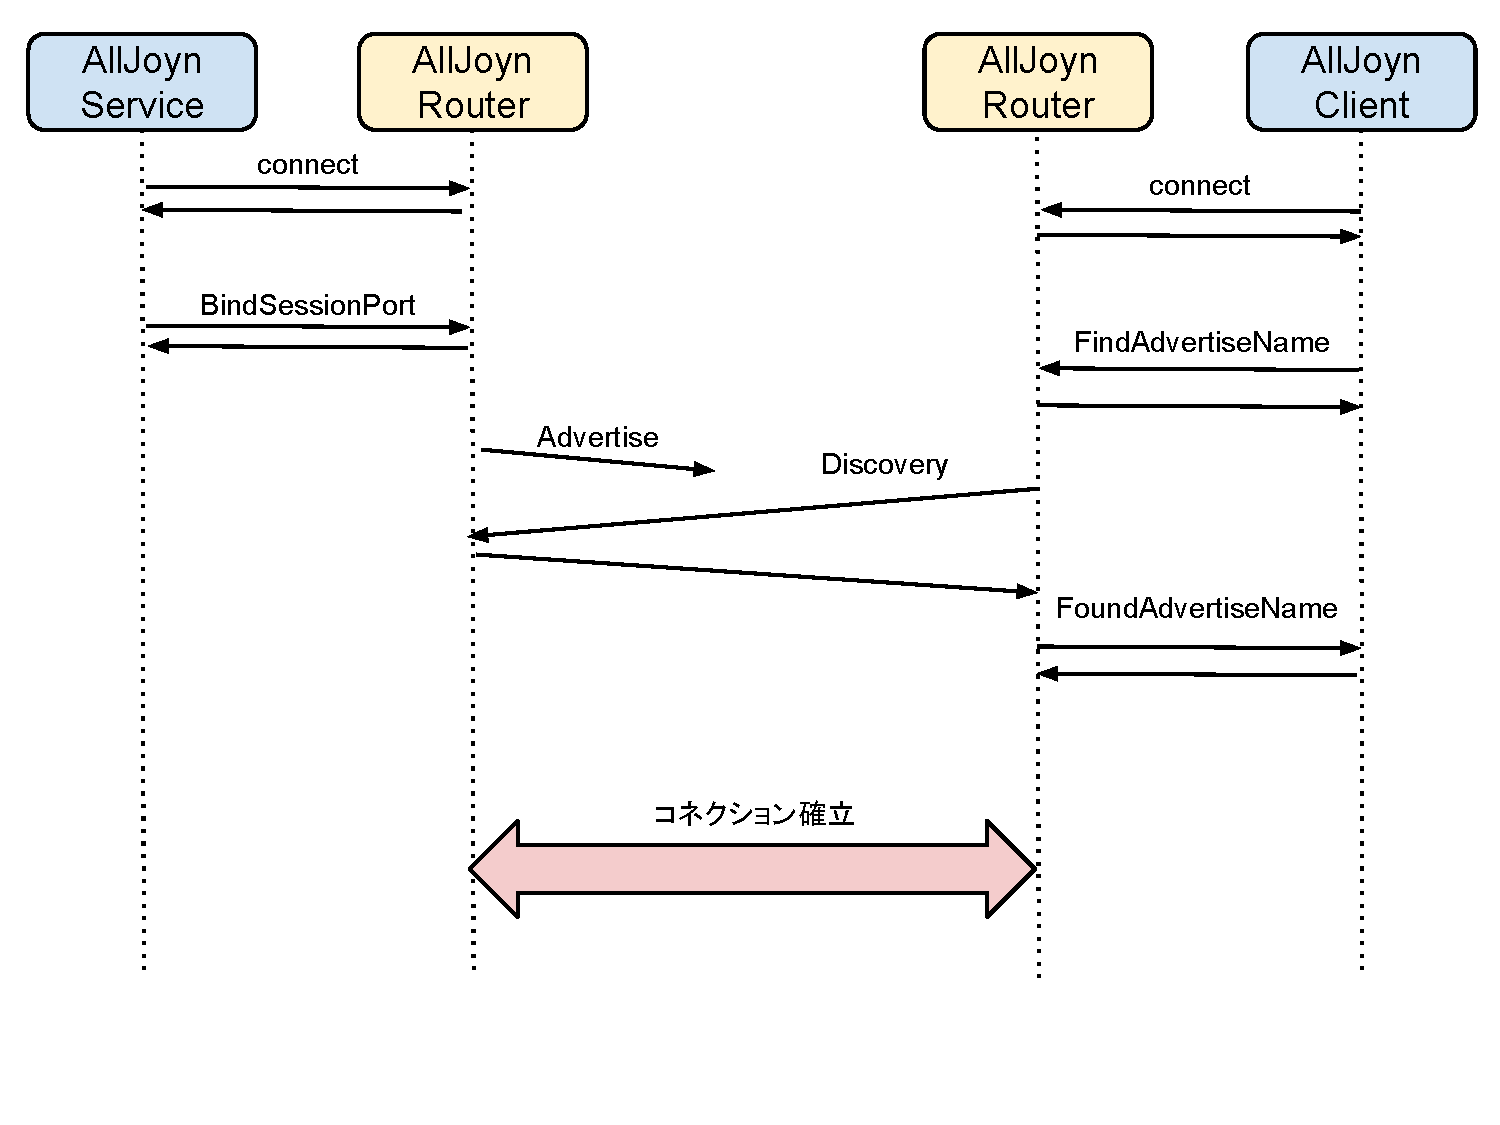
\includegraphics[width=10cm]{fig/AllJoyn_Session.pdf}
\caption{AllJoynセッションの例}
\end{figure}

\begin{enumerate}
\item AllClientとAllJoynServiceは,それぞれのAllJoyn Routerに接続する.
\item AllJoynServiceでは,BindSessionPort APIを用いてセッションポートやセッションオプションなどを決定する.
\item AllJoynServiceでは,AllJoyn Routerを通して任意の名前をAdvertiseしてコネクションを待つ.
\item AllJoynClientでは,AllJoyn Routerを通して任意の名前をDiscoverする.
\item Advertiseされている任意の名前と一致した場合,FoundAdvertiseNameシグナルがAllJoynClientに送られる.
\item AllJoynClientがJoinSession APIを用いてAllJoynClientとAllJoynServiceのコネクションが確立する.
\end{enumerate}


\subsection{iBeaconの検知}
iBeaconはiOS特有の機能であるが,Bluetooth Low Energy(BLE)を利用した技術であるため,BLEを受信することができるAndroid4.3以上かつBluetooth4.0に対応した端末ならiBeaconを検知することができる.
iBeaconがブロードキャストしているバイトデータは6$\sim$9バイト目が固定されており,この値を参照してiBeaconかどうかを判断する.

\begin{table}[htbp]
  \centering
  \begin{tabular}{|c|c|} \hline
    データ領域 & 説明 \\ \hline \hline
    1   & 1ブロック目のバイト数 \\ \hline
    2,3 & フラグ \\ \hline
    4   & 2ブロック目のバイト数 \\ \hline
    5   & メーカー固有のAD typeデータ \\ \hline
    6,7 & 会社コード(Appleのコードは0x004C) \\ \hline
    8   & データタイプ(iBeaconは0x02) \\ \hline
    9   & 連なるiBeaconデータのバイト数 \\ \hline
    10 $\sim$ 25 & UUID \\ \hline
    26,27 & major \\ \hline
    28,29 & minor \\ \hline
    30  & 受信強度を求めるための2の補数 \\ \hline
  \end{tabular}
  \caption{iBeaconデータ配列}
\end{table}

Androidアプリ内でバイトデータを処理し,UUIDやrssiといったビーコン情報を抽出する.


\subsection{プログラムファイル}
AllJoynAppは,
\begin{itemize}
\item AllJoynClient.java
\item AllJoynService.java
\item SimpleInterface.java
\end{itemize}
の三つのプログラムファイルから成る.


\begin{figure}[htbp]
\begin{center}
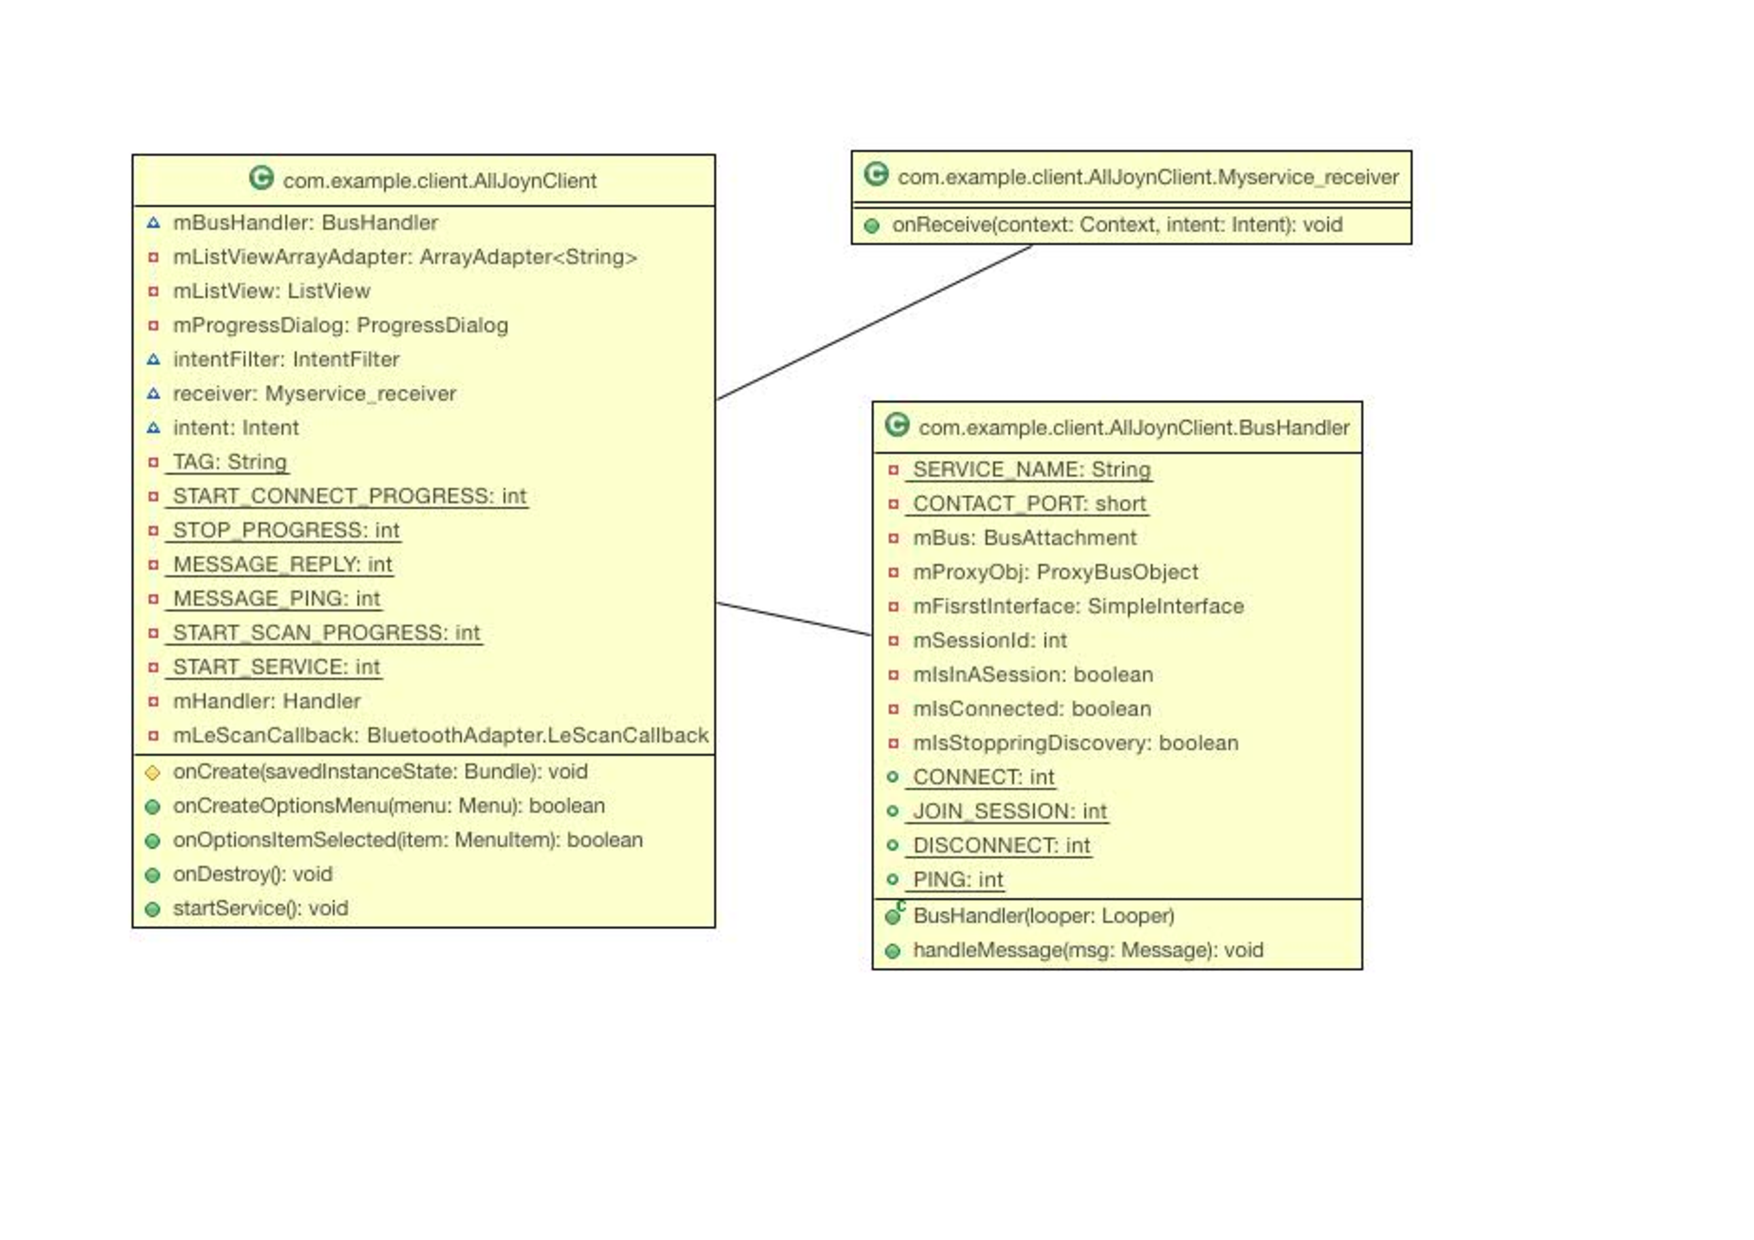
\includegraphics[width=10cm]{fig/class_client.pdf}
\end{center}
\caption{AllJoynClientクラス図}
\end{figure}

\begin{figure}
\begin{center}
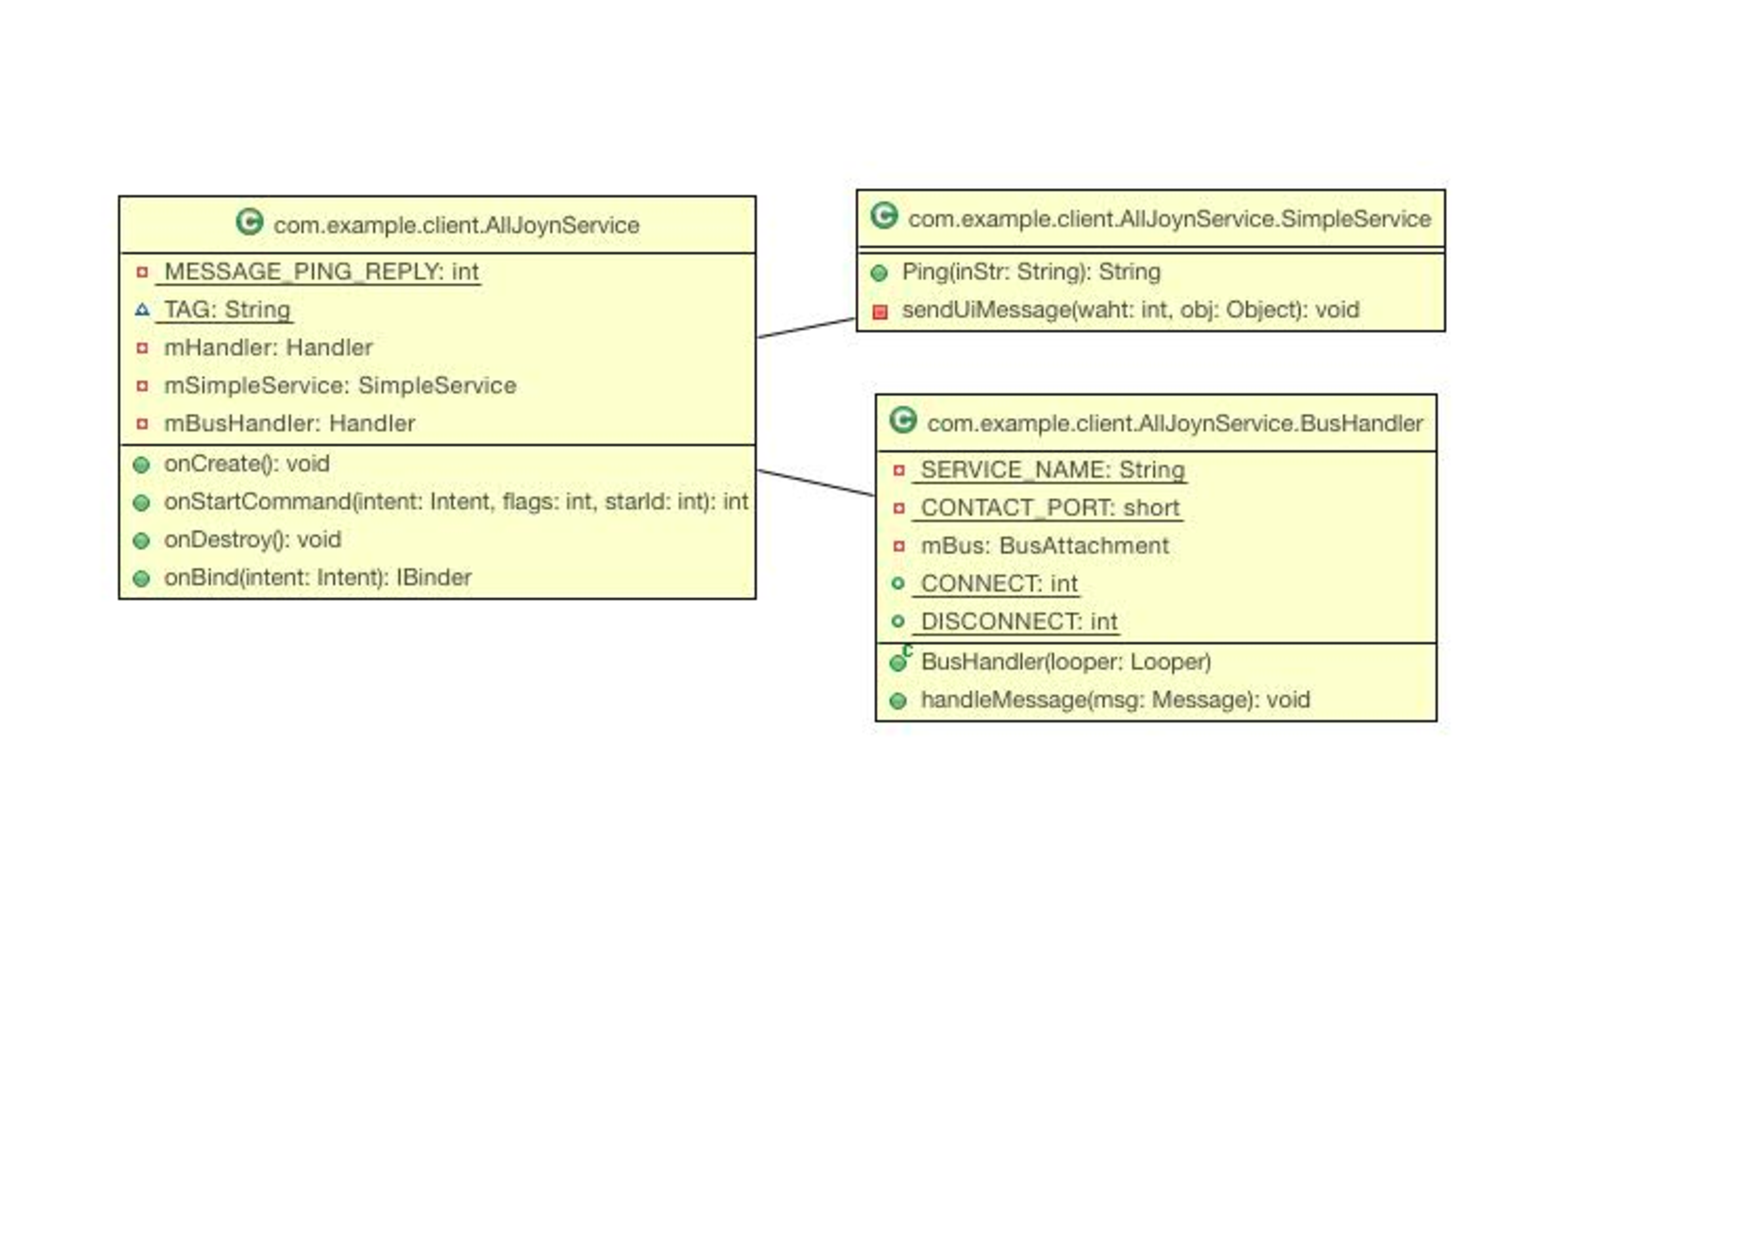
\includegraphics[width=10cm]{fig/class_service.pdf}
\end{center}
\caption{AllJoynServiceクラス図}
\end{figure}

\begin{figure}[htbp]
\centering
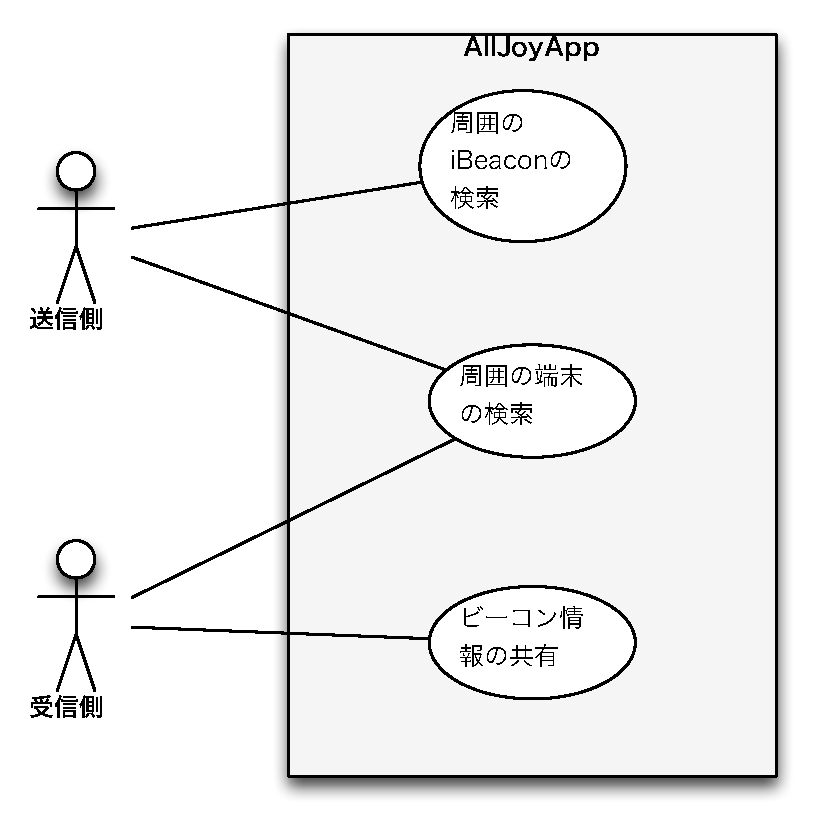
\includegraphics[width=7cm]{fig/usecase.pdf}
\caption{ユースケース図}
\end{figure}

\section{実装}
今回作成したAllJoynAppの処理を解説する.
操作の手順としては
\begin{enumerate}
\item アプリケーションの起動
\item FINDボタン押下
\item SCANボタン押下
\end{enumerate}
となっている.

\subsection{アプリケーションの起動}
アプリケーションを起動した際の処理は以下の通りである.

\begin{enumerate}
\item AllJoynClientを起動する.
\item AllJoynClientはAllJoynServiceを起動する.AllJoynServiceはバックグラウンドで動作する.
\item 画面上にFIND,SCANという二つのボタンを表示する.
\item AllJoynServiceはAllJoyn Routerと接続し,Advertiseする.
\end{enumerate}

\begin{figure}[htbp]
\centering
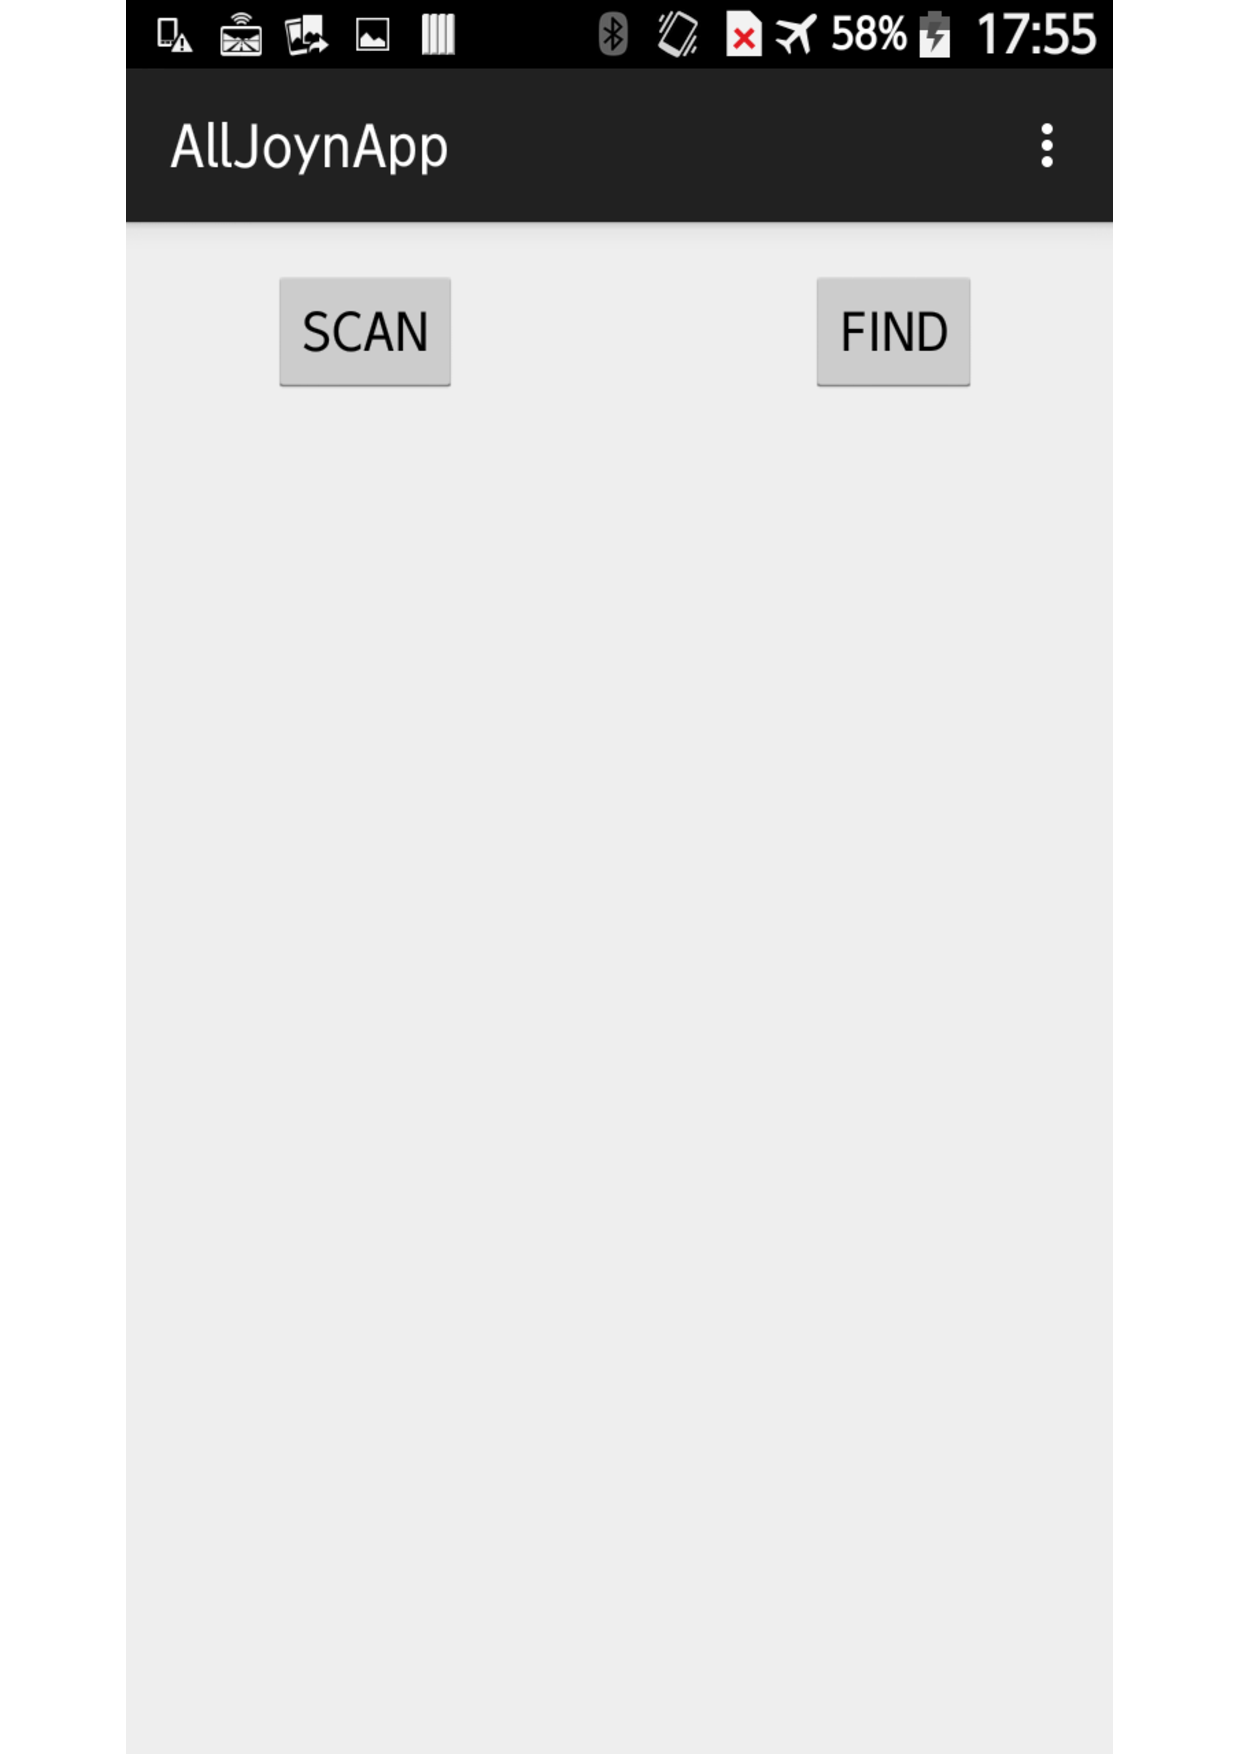
\includegraphics[width=5cm]{fig/screen1.pdf}
\caption{アプリケーション起動画面}
\end{figure}

以下の図は,端末A,端末BでAllJoynAppを起動した様子を表している.
端末A及び端末Bでは,AllJoynServiceが起動し,周囲にAdvertisementしている.

\begin{figure}[htbp]
\centering
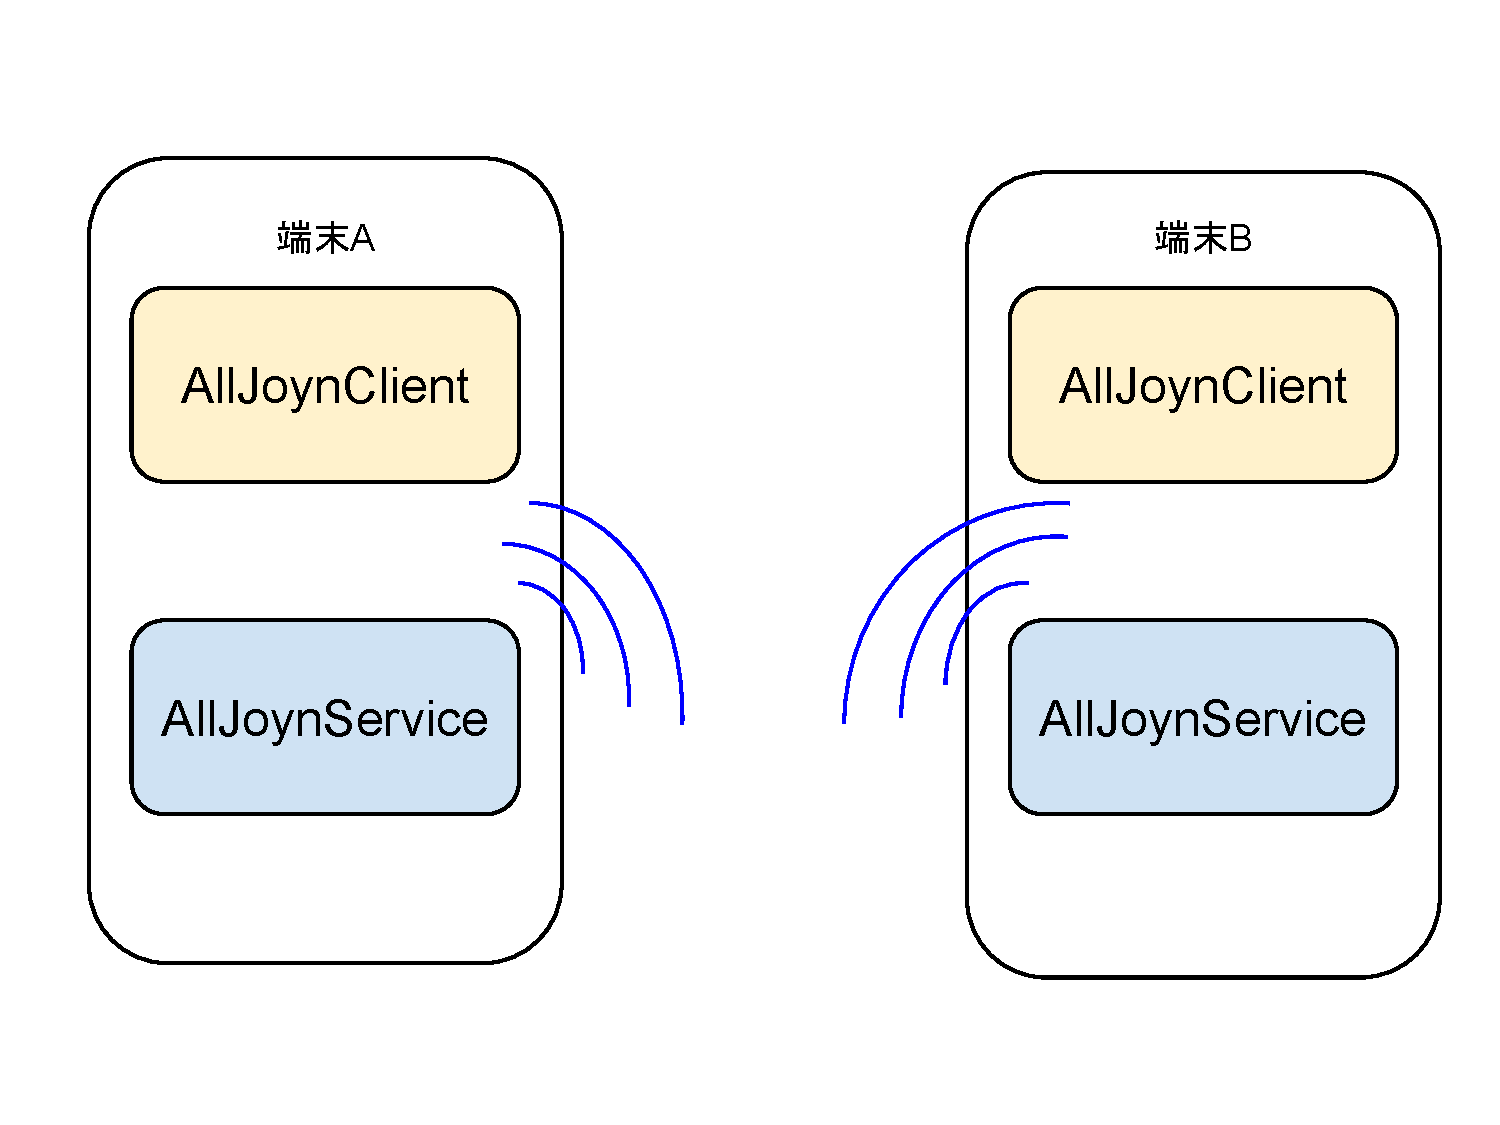
\includegraphics[width=10cm]{fig/appstart.pdf}
\caption{アプリケーション起動画面}
\end{figure}



\subsection{FINDボタン押下}
FINDボタンを押下した際の処理は以下の通りである.

\begin{enumerate}
\item 自身のAllJoynServiceを停止する.
\item AllJoynClientは自身のAllJoynRouterと接続する
\item 周囲のAllJoynServiceをDiscoveryする.
\item 検索している間,画面上には'DISCOVERING'と表示される
\item AllJoynServiceを検知した場合,コネクションを確立し,'DISCOVERING'の表示をやめる.
\end{enumerate}

同端末内でAllJoynClientとAllJoynServiceが起動している際,AllJoynClientは自身のAllJoynServiceと優先的に接続するため,Discoveryする前に自身のAllJoynServiceを停止させて周囲のAllJoynServiceをDiscoveryする.

\begin{figure}[htbp]
\centering
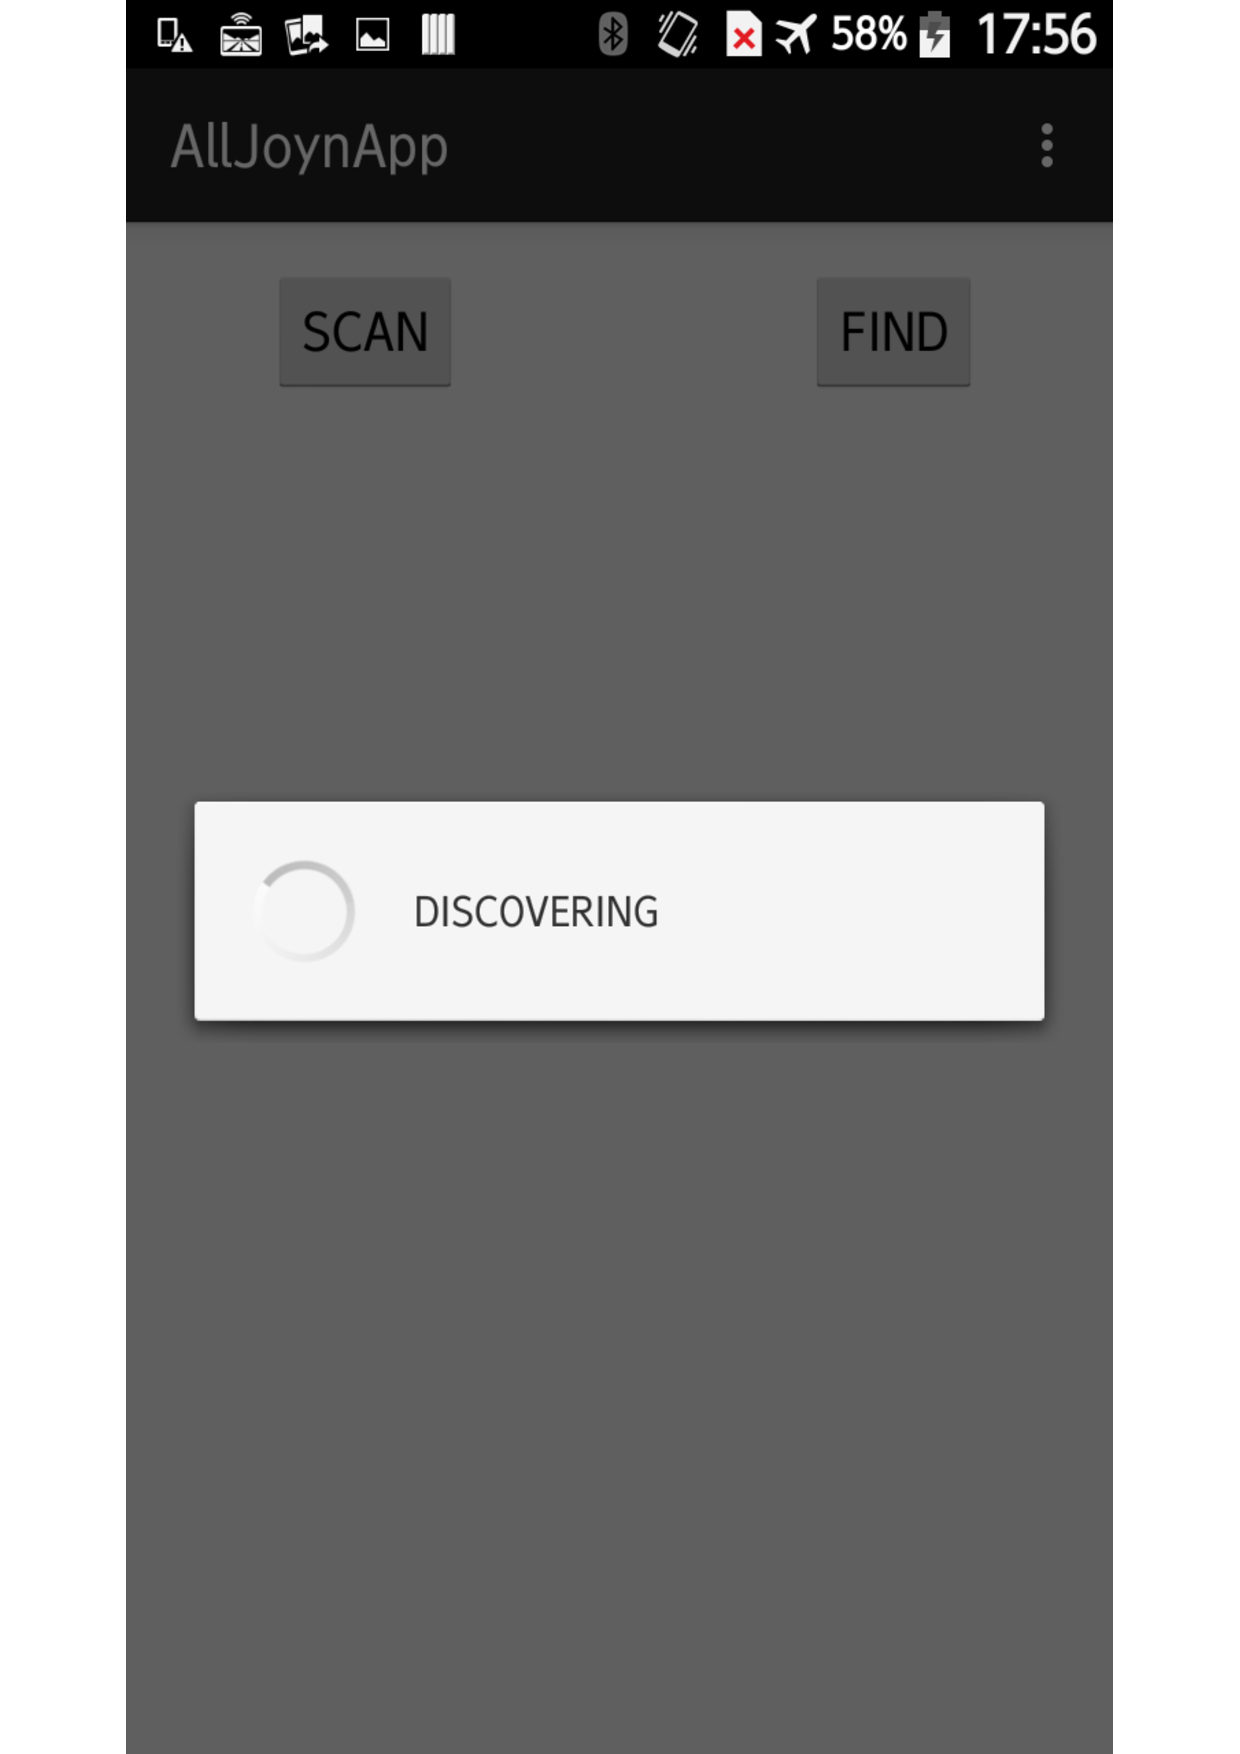
\includegraphics[width=5cm]{fig/screen2.pdf}
\caption{FINDボタン押下}
\end{figure}

以下の図では,端末AでFINDボタンを押下した際の様子を表している.
端末AではAllJoynServiceが停止し,端末AのAllJoynClientは端末BのAllJoynServiceとコネクションを確立させる.

\begin{figure}[htbp]
\centering
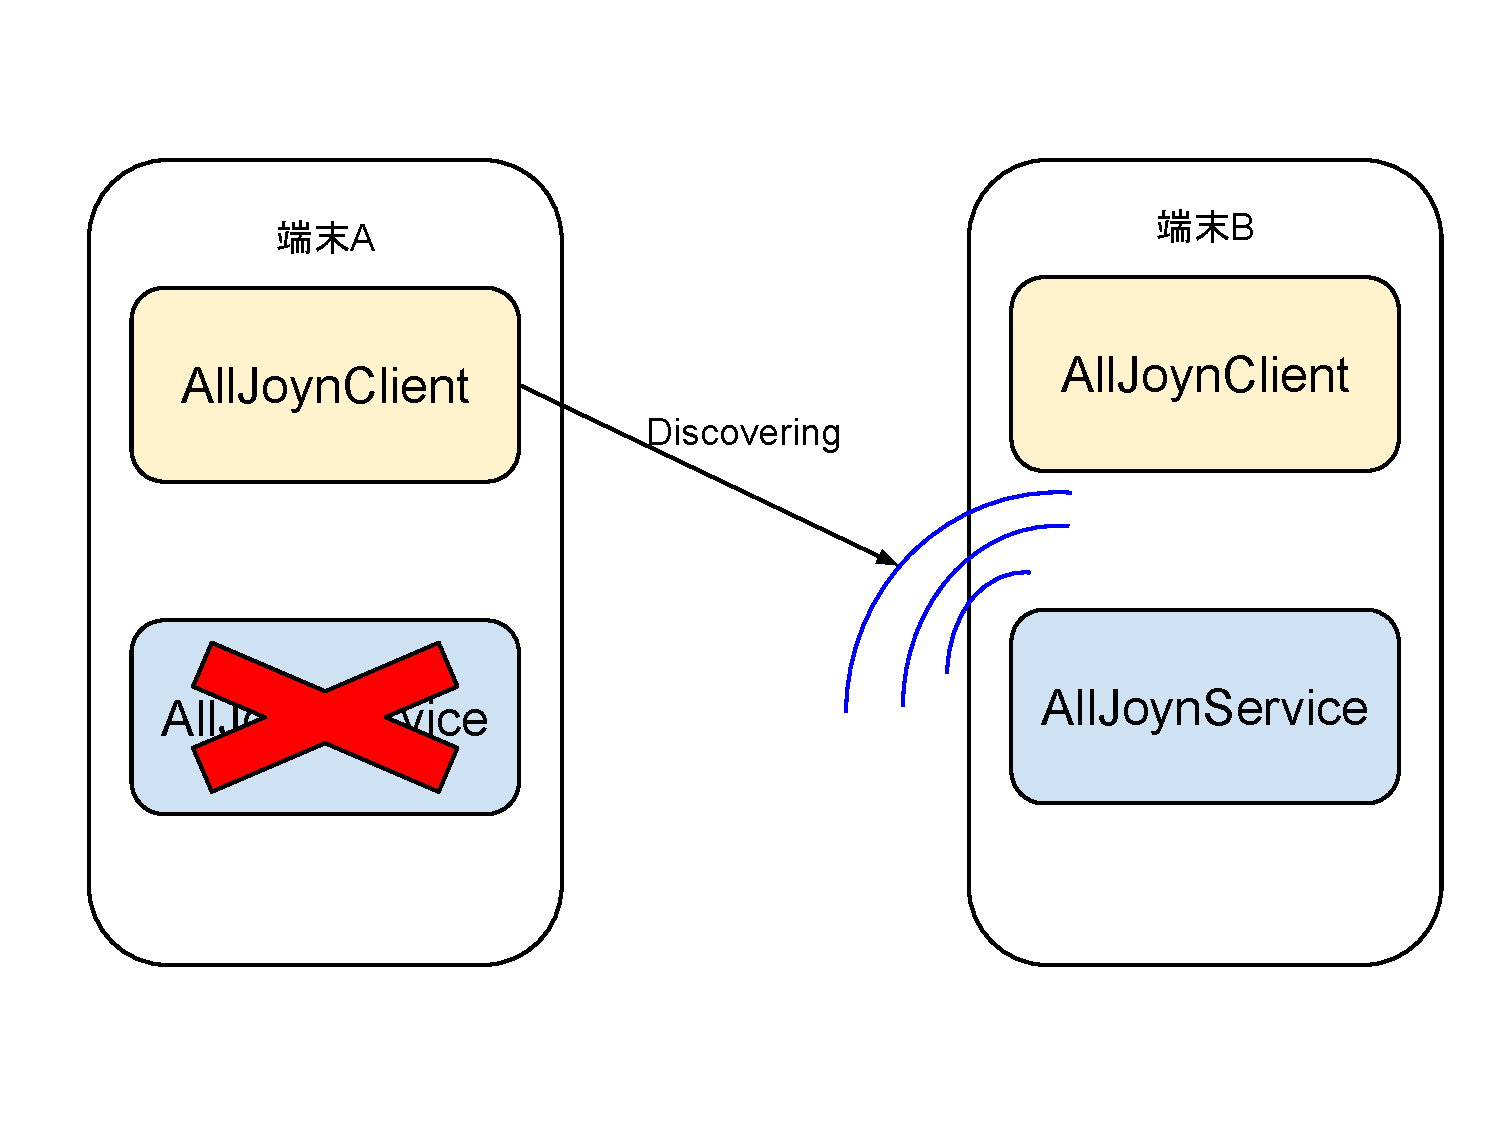
\includegraphics[width=10cm]{fig/click_find.pdf}
\caption{FINDボタン押下}
\end{figure}

\newpage

\subsection{SCANボタン押下}
SCANボタンが押下された際の処理は以下の通りである.
\begin{enumerate}
\item 二秒間周囲のiBeaconを検知し,ビーコン情報を画面上に表示する.iBeaconを検知しなかった場合,画面上に'iBeacon not found'と表示する.
\item AllJoynClientから,接続しているAllJoynServiceにビーコン情報を送信する.
\item ビーコン情報を受信したAllJoynServiceは,自身のAllJoynClientにビーコン情報を送信する.
\item AllJoynClientは,受信したビーコン情報を画面上に表示する.
\item 自身のAllJoynServiceを起動する.
\end{enumerate}


\begin{figure}[htbp]
\centering
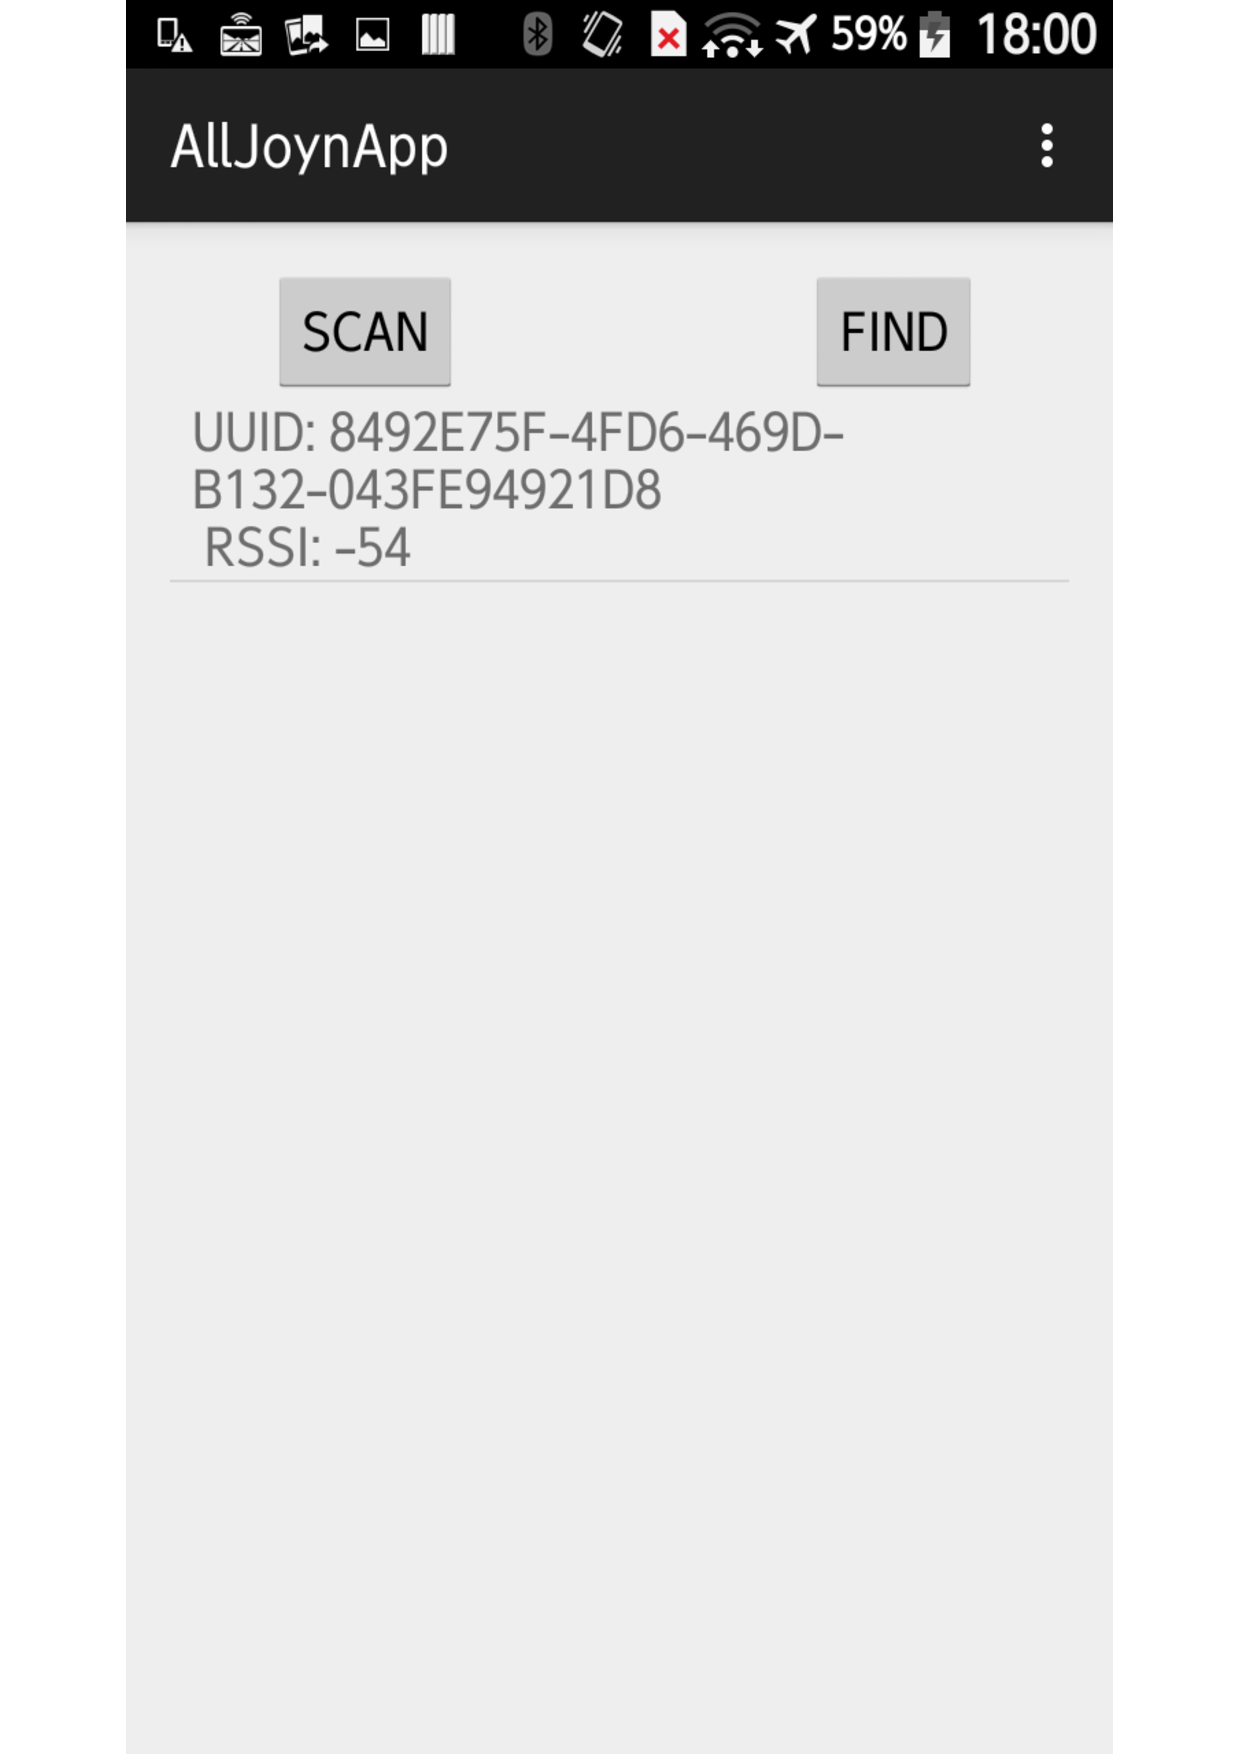
\includegraphics[width=5cm]{fig/screen3.pdf}
\caption{SCANボタン押下}
\end{figure}

以下の図は端末AでSCANボタンを押下した際の様子を表している.
端末AのAllJoynClientでビーコンを検知し,端末BのAllJoynServiceにビーコン情報を送信する.端末BのAllJoynServiceは自身のAllJoynClientにビーコン情報を送信し,画面上に表示する.

\begin{figure}[htbp]
\centering
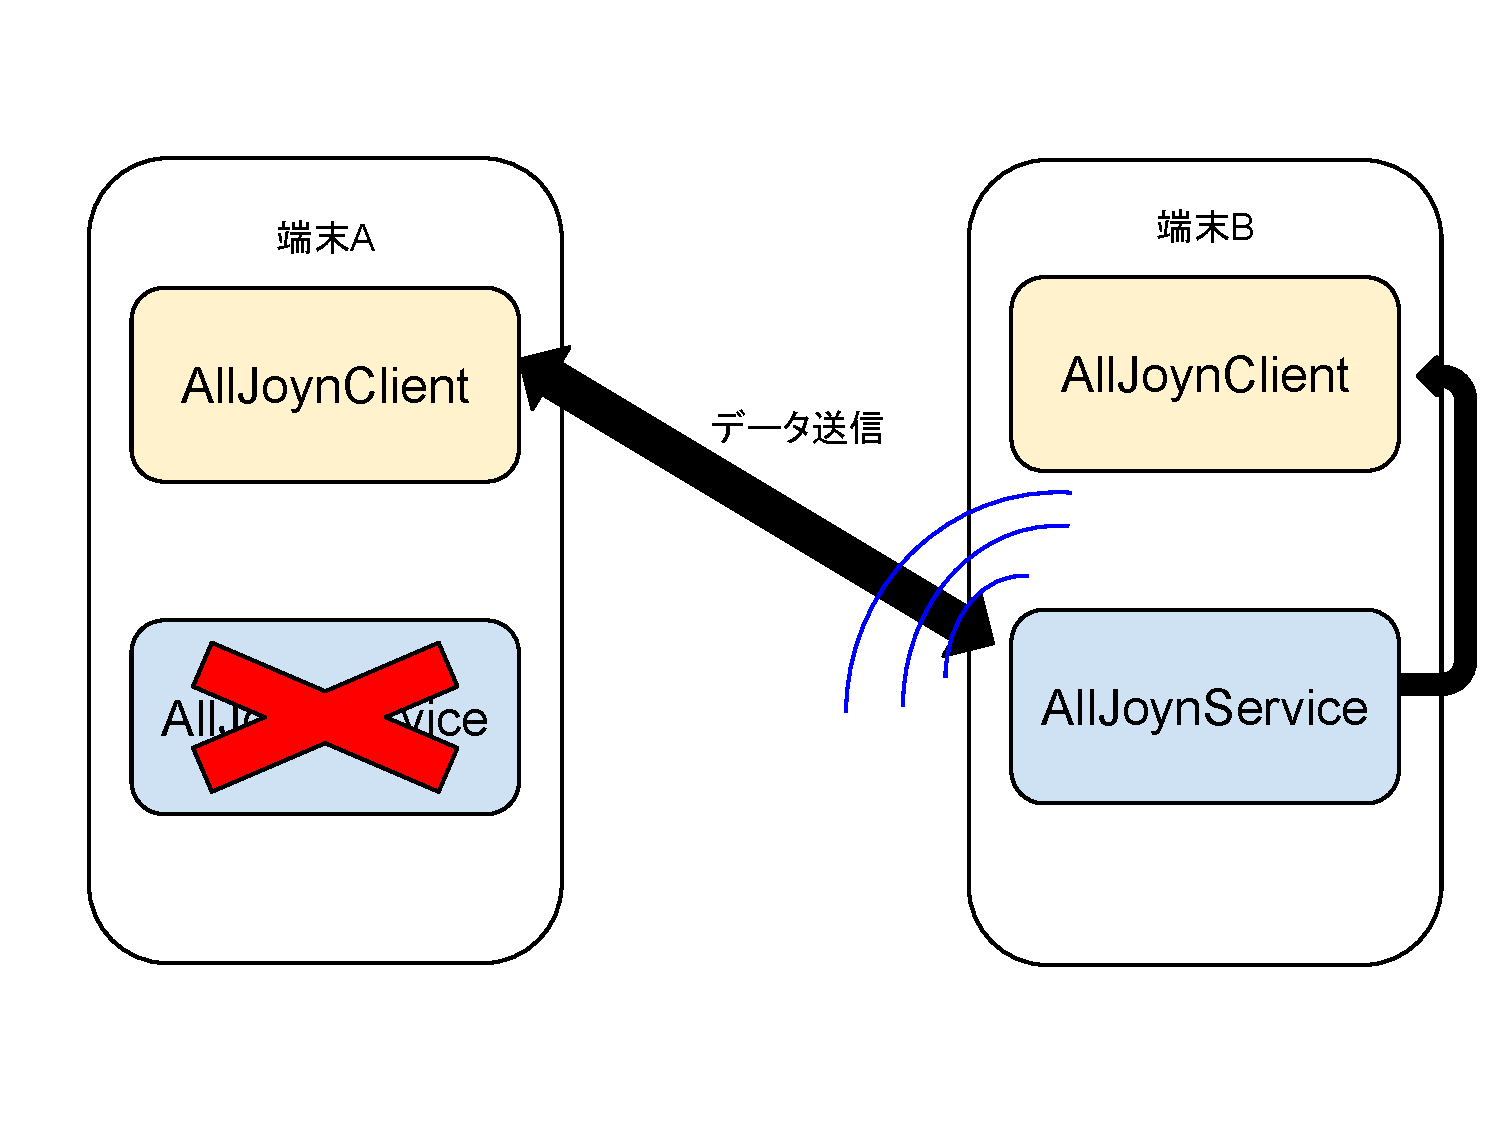
\includegraphics[width=10cm]{fig/click_scan.pdf}
\caption{SCANボタン押下}
\end{figure}




